
\chapter{Magnetism}

\begin{figure}[ht]
  \vspace{-40pt}
  \begin{centering}
      \fbox{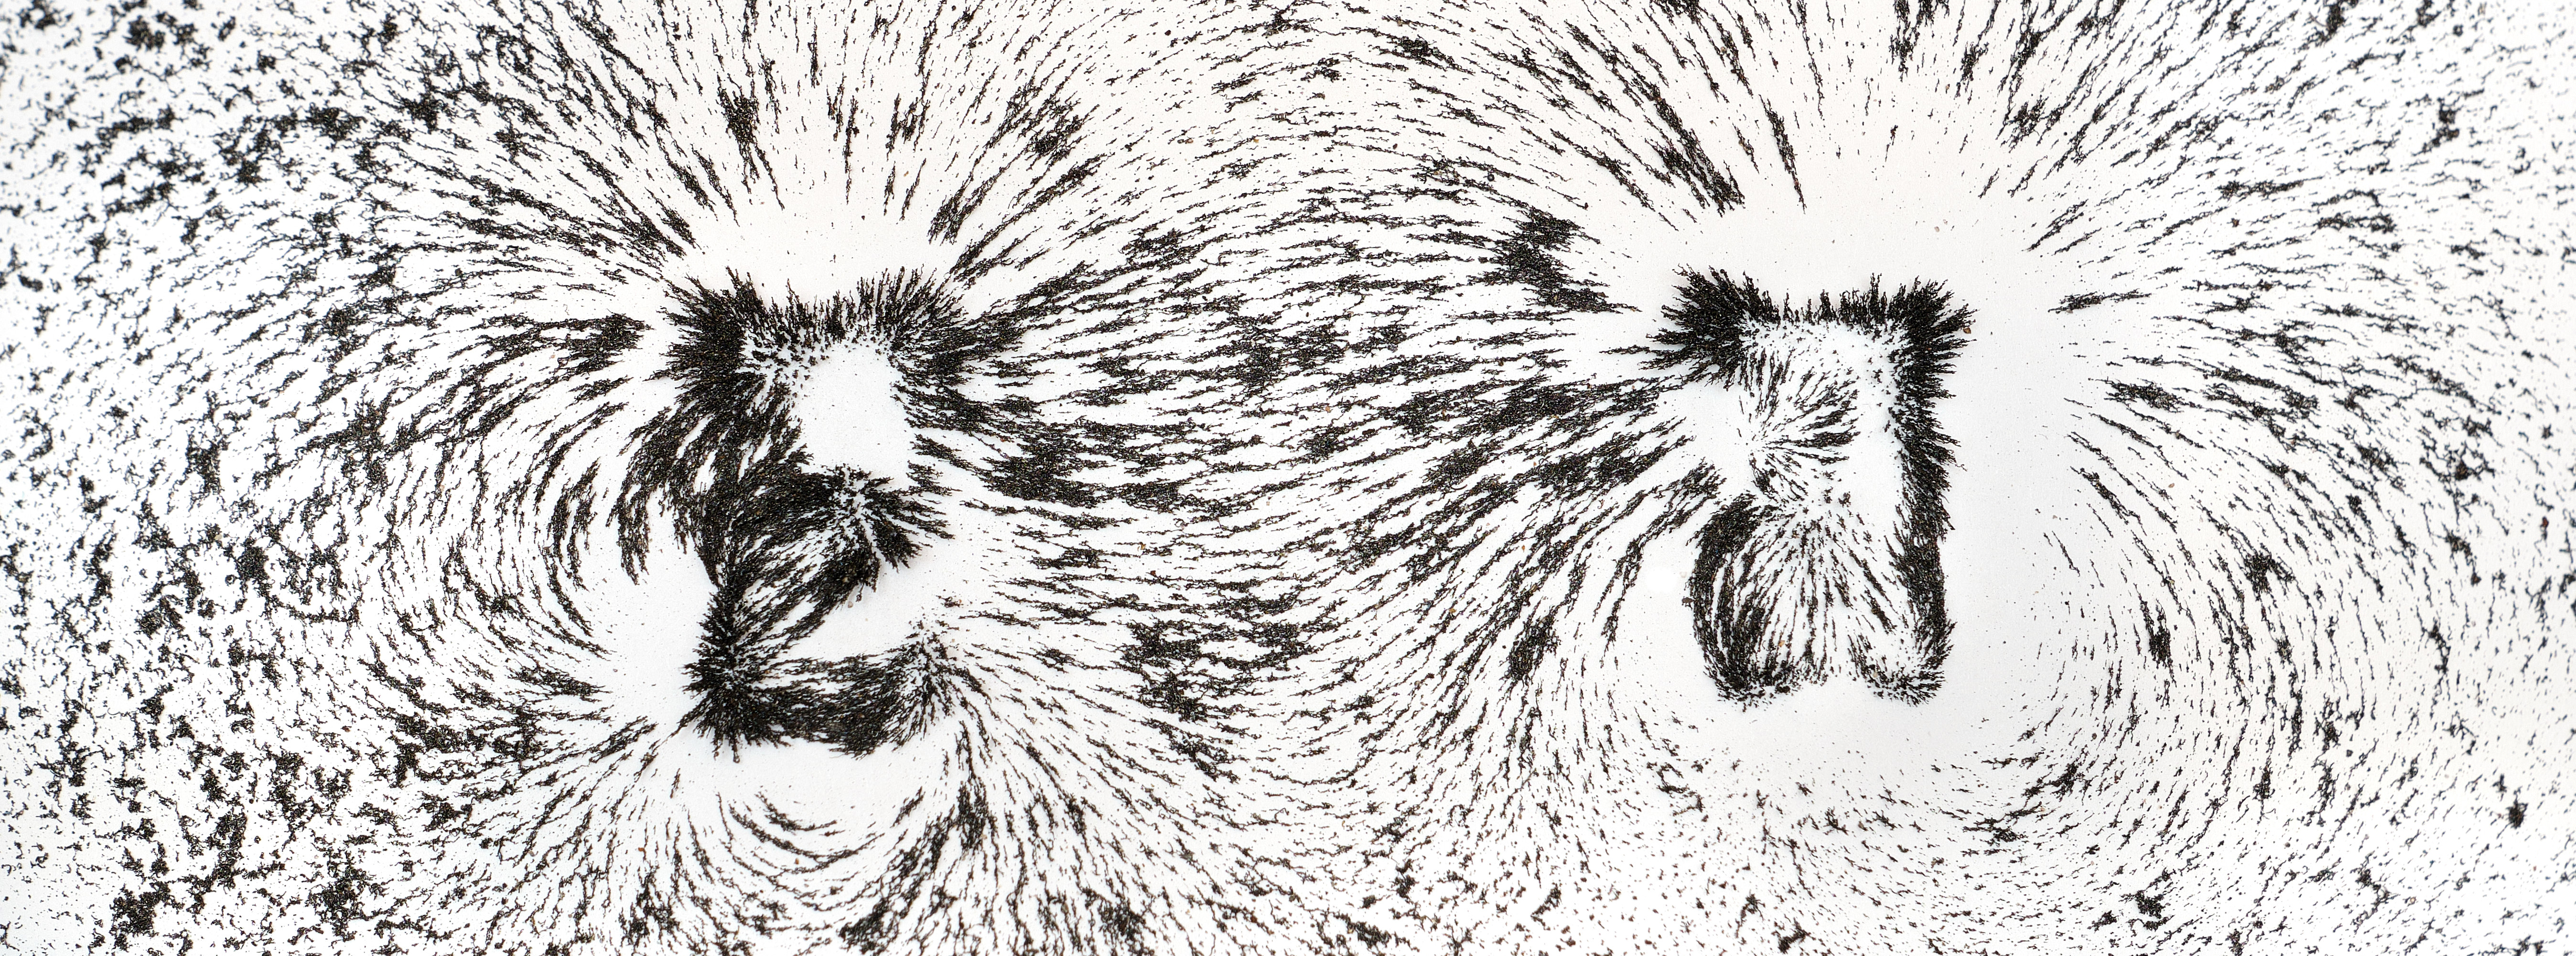
\includegraphics[width=\linewidth,height=.225\paperheight]{../../pictures/Horseshoe_magnet_metal_shavings_(top).jpg}}
      \caption{\footnotesize W.C. Woodbridge, \emph{Isothermal Chart} (1823). Public domain.}
  \end{centering}
\end{figure}
\clearpage

\lettrine[lines=4]{\goudy   I}{} have described the internal heat of our planet, both with reference to its cause and distribution, almost solely from the results of Fourier's admirable investigations. Poisson doubts the fact of the uninterrupted increase of the Earth's heat from the surface to the center, and is of the opinion that all heat has penetrated from without inward, and that the temperature of the globe depends upon the very high or very low temperature of the regions of space through which the solar system has moved. This hypothesis, imagined by one of the most acute mathematicians of our time, has not satisfied physicists or geologists, or scarcely, indeed, anyone besides its author. But, whatever may be the cause of the internal heat of our planet, and of its limited or unlimited increase in deep strata, it leads us, in this general sketch of nature, through the intimate connection of all primitive phenomena of matter, and through the common bond by which molecular forces are united, into the mysterious domain of magnetism. Changes of temperature call forth magnetic and electric currents. Terrestrial magnetism, whose main character, expressed in the threefold manifestation of its forces, is incessant periodic variability, is ascribed either to the heated mass of the Earth itself,\footnote{William Gilbert, of Colchester, whom Galileo pronounced "great," said "magnus magnes ipse est globus terrestris." He ridicules the magnetic mountains of Frascatori, the great contemporary of Columbus, as being magnetic poles "rejicienda est vulgaris opinio de montibus magneticis, aut rupe aliqua magnetica, aut polo phantastico a polo mundi distante." He assumes the declination of the magnetic needle at any given point on the surface of the Earth to be invariable ("variatio uniuscujusque loci constans est"), and refers the curvatures of the isogonic lines to the configuration of continents and the relative positions of sea basins, which possess a weaker magnetic force than the solid masses rising above the ocean. (Gilbert, de Magnete, ed. 1633, p. 42, 98, 152, and 155.)} or to those galvanic currents which we consider as electricity in motion, that is, electricity moving in a closed circuit.\footnote{Gauss, Allgemeine Theorie des Erdmagnetismus, in the Resultate aus den Beob. des Magnet. Vereins, 1838, s. 41, p. 56.}

The mysterious course of the magnetic needle is equally affected by time and space, by the sun's course, and by changes of place on the Earth's surface. Between the tropics, the hour of the day may be known by the direction of the needle as well as by the oscillations of the barometer. It is affected instantly, but only transiently, by the distant northern light as it shoots from the pole, flashing in beams of colored light across the heavens. When the uniform horary motion of the needle is disturbed by a magnetic storm, the perturbation manifests itself simultaneously, in the strictest sense of the word, over hundreds and thousands of miles of sea and land, or propagates itself by degrees, in short intervals of time, in every direction over the Earth's surface.\footnote{There are also perturbations which are of a local character, and do not extend themselves far, and are probably less deep-seated. Some years ago I described a rare instance of this kind, in which an extraordinary disturbance was felt in the mines at Freiberg, but was not perceptible at Berlin. (Lettre de M. de Humboldt  Son Altesse Royale le Duc de Sussex sur les moyens propres  perfectionner la Connaissance du Magn\'{e}tisme Terrestre, in Becquerel's T'rait\'{e} Exp\'{e}rimental del Elecsricit\'{e}, t. vii., p. 442.) Magnetic storms, which were simultaneously felt from Sicily to Upsala, did not extend from Upsala to Alten. (Gauss and Weber, Resultate des Magnet. Vereins, 1839,  128; Lloyd, in the Comptes Rendus de l'Acad. des Sciences, t. xiii., 1843, S\'{e}m. 11., p. 725 and 827.) Among the numerous examples that have been recently observed, of perturbations occurring simultaneously and over wide portions of the Earth's surface, and which are collected in Sabine's important work (Observ. on Days of unusual Magnetic Disturbance, 1843), one of the most remarkable is that of the 25th of September, 1841, which was observed at Toronto in Canada, at the Cape of Good Hope, at Prague, and partially in Van Diemen's Land. The English Sunday, on which it is deemed sinful, after midnight on Saturday, to register an observation, and to follow out the great phenomena of creation in their perfect development, interrupted the observations in Van Diemen's Land, where, in consequence of the difference of the longitude, the magnetic storm fell on the Sunday. (Observ., p. xiv., 78, 85, and 87.)} In the former case, the simultaneous manifestation of the storm may serve, within certain limitations, like Jupiter's satellites, fire signals, and well-observed falls of shooting stars, for the geographical determination of degrees of longitude. We here recognize with astonishment that the perturbations of two small magnetic needles, even if suspended at great depths below the surface, can measure the distances apart at which they are placed, teaching us, for instance, how far Kasan is situated east of G\"{o}ttingen or of the banks of the Seine. There are also districts in the earth where the mariner, who has been enveloped for many days in mist, without seeing either the sun or stars, and deprived of all means of determining the time, may know with certainty, from the variations in the inclination of the magnetic needle, whether he is at the north or the south of the port he is desirous of entering.\footnote{I have described, in Lam\'{e}therie's Journal de Physique, 1804, t.lix., p. 449, the application (alluded to in the text) of the magnetic inclination to the determination of latitude along a coast running north and south, and which, like that of Chili and Peru, is for a part of the year enveloped in mist (garua). In the locality I have just mentioned, this application is of the greater importance, because, in consequence of the strong current running northward as far as to Cape Parefia, navigators incur a great loss of time if they approach the coast to the north of the haven they are seeking. In the South Sea, from Callao de Lima harbor to Truxillo, which differ from each other in latitude by $3^{\circ} 57^{\prime}$, I have observed a variation of the magnetic inclination amounting to 9 (centesimal division); and from Callao to Guayaquil, which differ in latitude by $9^{\circ} 50^{\prime}$, a variation of $23^{\circ} 95^{\prime}$. (See my Relat. Hist., t. iii., p. 622.) At Guarmey ($10^{\circ} 4^{\prime}$ south lat.), Huaura ($11^{\circ} 3^{\prime}$ south lat.), and Chancay ($11^{\circ} 32^{\prime}$ south lat.), the inclinations are $69^{\circ} 80^{\prime}$, $99^{\circ}$, and $103^{\circ} 5^{\prime}$ of the centesimal division. The determination of position by means of the magnetic inclination has this remarkable feature connected with it, that where the ship's course cuts the isoclinal line almost perpendicularly, it is the only one that is independent of all determination of time, and, consequently, of observations of the sun or stars. It is only lately that I discovered, for the first time, that as early as at the close of the sixteenth century, and consequently hardly twenty years after Robert Norman had invented the inclinatorium, William Gilbert, in his great work De Magnete, proposed to determine the latitude by the inclination of the magnetic needle. Gilbert (Physiologia Nova de Magnete, lib. v., cap. 8, p. 200) commends the method as applicable a\'{e}re caliginoso. Edward Wright, in the introduction which he added to his master's great work, describes this proposal as "worth much gold." As he fell into the same error with Gilbert, of presuming that the isoclinal lines coincided with the geographical parallel circles, and that the magnetic and geographical equators were identical, he did not perceive that the proposed method had only a local and very limited application.}

When the needle, by its sudden disturbance in its horary course, indicates the presence of a magnetic storm, we are still unfortunately ignorant whether the seat of the disturbing cause is to be sought in the Earth itself or in the upper regions of the atmosphere. If we regard the Earth as a true magnet, we are obliged, according to the views entertained by Friedrich Gauss (the acute propounder of a general theory of terrestrial magnetism), to ascribe to every portion of the globe measuring one eighth of a cubic meter (or $3\frac{7}{10}$ths of a French cubic foot) in volume, an average amount of magnetism equal to that contained in a magnetic rod of 1 lb. weight.\footnote{Gauss and Weber, Resultate des Magnet. Vereins, 1838, 31, s. 146.} If iron and nickel, and probably, also, cobalt (but not chrome, as has long been believed),\footnote{According to Faraday (London and Edinburgh Philosophical Magazine, 1836, vol. viii., p. 178), pure cobalt is totally devoid of magnetic power. I know, however, that other celebrated chemists (Heinrich Rose and W\'{e}hler) do not admit this as absolutely certain. If out of two carefully purified masses of cobalt totally free from nickel, one appears altogether nonmagnetic (in a state of equilibrium), I think it probable that the other owes its magnetic property to a want of purity; and this opinion coincides with Faraday's view.} are the only substances which become permanently magnetic and retain polarity from a certain coercive force, the phenomena of Arago's magnetism of rotation and of Faraday's induced currents show, on the other hand, that all telluric substances may possibly be made transitorily magnetic. According to the experiments of the first mentioned of these great physicists, water, ice, glass, and carbon affect the vibrations of the needle entirely in the same manner as mercury in the rotation experiments.\footnote{Arago, in the Annales de Chimie, t. xxxii., p.214; Brewster, J'reatise on Magnetism, 1837, p. 111; Baumgartner, in the Zeitschrift furPhys. und Mathem., bd. ii., s. 419.} Almost all substances show themselves to be, in a certain degree, magnetic when they are conductors, that is to say, when a current of electricity is passing through them.

Although the knowledge of the attracting power of native iron magnets or loadstones appears to be of very ancient date among the nations of the West, there is strong historical evidence in proof of the striking fact that the knowledge of the directive power of a magnetic needle and of its relation to terrestrial magnetism was peculiar to the Chinese, a people living in the easternmost portions of Asia. More than a thousand years before our era, in the obscure age of Codrus, and about the time of the return of the Heraclidae to the Peloponnesus, the Chinese had already magnetic carriages, on which the movable arm of the figure of a man continually pointed to the south, as a guide by which to find the way across the boundless grass plains of Tartary; nay, even in the third century of our era, therefore at least 700 years before the use of the mariners compass in European seas, Chinese vessels navigated the Indian Ocean\footnote{Humboldt, Examen Critique de l'Hist. de la Géographie, t. iii., p. 36.} under the direction of magnetic needles pointing to the south. I have shown, in another work, what advantages this means of topographical direction, and the early knowledge and application of the magnetic needle gave the Chinese geographers over the Greeks and Romans, to whom, for instance, even the true direction of the Apennines and Pyrenees always remained unknown.\footnote{Asiatic Researches, t. i., Introduction, p. xxxviii-xlii. The Western nations, the Greeks and the Romans, knew that magnetism could be communicated to iron, and that the metal would retain it for a length of time. (Sola hec materia ferri vires, a magnete lapide accipit, retinezque longo tempore. Plin., xxxiv.,14.) The great discovery of the terrestrial directive force depended, therefore, alone on this, that no one in the West had happened to observe an elongated fragment of magnetic iron stone, or a magnetic iron rod, floating, by the aid of a piece of wood, in water, or suspended in the air by a thread, in such a position as to admit of free motion.}

The magnetic power of our globe is manifested on the terrestrial surface in three classes of phenomena, one of which exhibits itself in the varying intensity of the force, and the two others in the varying direction of the inclination, and in the horizontal deviation from the terrestrial meridian of that spot. Their combined action may therefore be graphically represented by three systems of lines, the isodynamic, isoclinic, and isogonic (or those of equal force, equal inclination, and equal declination). The distances apart, and the relative positions of these moving, oscillating, and advancing curves, do not always remain the same. The total deviation (variation or declination of the magnetic needle) has not at all changed, or, at any rate, not in any appreciable degree, during a whole century, at any particular point on the Earth's surface,\footnote{A very slow secular progression, or a local invariability of the magnetic declination, prevents the confusion which might arise from terrestrial influences in the boundaries of land, when, with an utter disregard for the correction of declination, estates are, after long intervals, measured by the mere application of the compass. The whole mass of West Indian property, says Sir John Herschel, has been saved from the bottomless pit of endless memories by the invariability of the magnetic declination in Jamaica and the surrounding Archipelago during the whole of the last century, all surveys of property there having been conducted solely by the compass. See Robertson, in the Philosophical Transactions for 1806, Part ii., p. 348, On the Permanency of the Compass in Jamaica since 1660. In the mother country (England) the magnetic declination has varied by fully 14 during that period.} as, for instance, the western part of the Antilles, or Spitzbergen. In like manner, we observe that the isogonic curves, when they pass in their secular motion from the surface of the sea to a continent or an island of considerable extent, continue for a long time in the same position, and become inflected as they advance.

These gradual changes in the forms assumed by the lines in their translatory motions, and which so unequally modify the amount of eastern and western declination, in the course of time render it difficult to trace the transitions and analogies of forms in the graphic representations belonging to different centuries. Each branch of a curve has its history, but this history does not reach further back among the nations of the West than the memorable epoch of the 13th of September, 1492, when the rediscoverer of the New World found a line of no variation 3 west of the meridian of the island of Flores, one of the Azores.\footnote{I have elsewhere shown that, from the documents which have come down to us regarding the voyages of Columbus, we can, with much certainty, fix upon three places tm the Atlantic line of no declination for the 13th of September, 1492, the 2ist of May, 1496, and the 16th of August, 1498. The Atlantic line of no declination at that period ran from northeast to southwest. It then touched the foutk American continent a little east of Cape Codera, while it is now observed to reach that continent on the northern coast of the Brezik (Humboldt, Ezamen Critique de l Hist. de la G\'{e}ogr., t. iii., p. 44 - 48 From Gilberts Phystologia Nova de Magnete, we see plainly (and the fact is very remarkable) that in 1600 the declination was still null in the region of the Azores, just as it had been in the time of Columbus (lib. 4, cap. 1). I believe that in my Examen Critique (t. iii., p. 54) I have proved from documents that the celebrated line of demarkation by which Pope Alexander VI. divided the Western hemisphere between Portugal and Spain was not drawn through the most western point of the Azores, because Columbus wished to convert a physical into a political division. He attached great importance to the zone (raya) sci) which the compass shows no variation, where air and ocean, the latter covered with pastures of seaweed, exhibit a peculiar constitution, where cooling winds begin to blow, and where as erroneous observations of the polar star led him to imagine the form (sphericity) of the Earth is no longer the same.} The whole of Europe, excepting a small part of Russia, has now a western declination, while at the close of the seventeenth century the needle first pointed due north, in London in 1657, and in Paris in 1669, there being thus a difference of twelve years, notwithstanding the small distance between these two places. In Eastern Russia, to the east of the mouth of the Volga, of Saratow, Nischni Nowgorod, and Archangel, the easterly declination of Asia is advancing toward us. T'wo admirable observers, Hansteen and Adolphus Erman, have made us acquainted with the remarkable double curvature of the lines of declination in the vast region of Northern Asia; these being concave toward the pole between Obdorsk, on the Oby, and Turuchansk, and convex between the Lake of Baikal and the Gulf of Ochotsk. In this portion of the earth, in northern Asia, between the mountains of Werchojansk, Jakutsk, and the northern Korea, the isogonic lines form a remarkable closed system. This oval configuration\footnote{To determine whether the two oval systems of isogonic lines, so singularly included each within itself, will continue to advance for centuries in the same enclosed form, or will unfold and expand themselves, is a question of the highest interest in the problem of the physical causes of terrestrial magnetism. In the Eastern Asiatic nodes the declination increases from without inward, while in the node or oval system of the South Sea the opposite holds good; in fact, at the present time, in the whole South Sea to the east of the meridian of Kamtschatka, there is no line where the declination is null, or, indeed, in which it is less than 2 (Erman, in Pogg., Annal., bd. xxxi., 129). Yet Cornelius Schouten, on Easter Sunday, 1616; appears to have found the declination null somewhere to the southeast of Nukahiva, in 15 south lat. and 132 west long., and consequently in the middle of the present closed isogonal system. (Hansteen, Magnet. der Erde, 1819, 28.) It must not be forgotten, in the midst of all these considerations, that we can only follow the direction of the magnetic lines in their progress as they are projected upon the surface of the Earth.} recurs regularly, and over a great extent of the South Sea, almost as far as the meridian of Pitcairn and the group of the Marquesas Islands, between 20 north and 45 south lat. One would almost be inclined to regard this singular configuration of closed, almost concentric, lines of declination as the effect of a local character of that portion of the globe; but if, in the course of centuries, these apparently isolated systems should also advance, we must suppose, as in the case of all great natural forces, that the phenomenon arises from some general cause.

The horary variations of the declination, which, although dependent upon true time, are apparently governed by the Sun, as long as it remains above the horizon, diminish in angular value with the magnetic latitude of place. Near the equator, for instance, in the island of Rawak, they scarcely amount to three or four minutes, while they are from thirteen to fourteen minutes in the middle of Europe. As in the whole northern hemisphere the north point of the needle moves from east to west on an average from 8:00 AM until 1:00 PM, while in the southern hemisphere the same north point moves from west to east.\footnote{Arago, in the Annuaire, 1836, p. 284, and 1840, p. 330-338.} Attention has recently been drawn, with much justice, to the fact that there must be a region of the Earth between the terrestrial and the magnetic equator where no horary deviations in the declination are to be observed. This fourth curve, which might be called the \emph{curve of no motion}, or, rather, \emph{the line of no variation of horary declination}, has not yet been discovered.

The term \emph{magnetic poles} has been applied to those points of the Earth's surface where the horizontal power disappears, and more importance has been attached to these points than properly appertains to them;\footnote{Gauss, Allg. Theorie des Erdmagnet.,  31.} and in like manner, the curve, where the inclination of the needle is null, has been termed the \emph{magnetic equator}. The position of this line and its secular change of configuration have been made an object of careful investigation in modern times. According to the admirable work of Duperrey,\footnote{Duperrey, De la Configuration de  Equateur Magn\'{e}tique, in the Annales de Chimie, t. xlv., p. 371 and 379. (See, also, Morlet, in the M\'{e}moires pr\'{e}sent\'{e}s par divers Savans a l Acat. Roy. des Sciences, t. iii. p 132.)} who crossed the magnetic equator six times between 1822 and 1825, the nodes of the two equators, that is to say, the two points at which the line without inclination intersects the terrestrial equator, and consequently passes from one hemisphere into the other, are so unequally placed, that in 1825 the node near the island of St. Thomas, on the western coast of Africa, was $188\frac{1}{2}^\circ$ distant from the node in the South Sea, close to the little islands of Gilbert, nearly in the meridian of the Viti group. In the beginning of the present century, at an elevation of 11,936 feet above the level of the sea, I made an astronomical determination of the point ($7^\circ 1^\prime$ south lat., $48^\circ 40^\prime$ west long. from Paris), where, in the interior of the New Continent, the chain of the Andes is intersected by the magnetic equator between Quito and Lima. To the west of this point, the magnetic equator continues to traverse the South Sea in the southern hemisphere, at the same time slowly drawing near the terrestrial equator. It first passes into the northern hemisphere a little before it approaches the Indian Archipelago, just touches the southern points of Asia, and enters the African continent to the west of Socotora, almost in the Straits of BabelMandeb, where it is most distant from the terrestrial equator. After intersecting the unknown regions of the interior of Africa in a southwest direction, the magnetic equator reenters the south tropical zone in the Gulf of Guinea, and retreats so far from the terrestrial equator that it touches the Brazilian coast near Os Ilheos, north of Porto Seguro, in 15 south lat. From thence to the elevated plateaux of the Cordilleras, between the silver mines of Micuipampa and Caxamarca, the ancient seat of the Incas, where I observed the inclination, the line traverses the whole of South America, which in these latitudes is as much a magnetic \emph{terra incognita} as the interior of Africa.

The recent observations of Sabine\footnote{See the remarkable chart of isoclinic lines in the Atlantic Ocean for the years 1825 and 1837, in Sabine's Contributions to Terrestrial Magnetism, 1840, p. 134.} have shown that the node near the island of St. Thomas has moved 4 from east to west between 1825 and 1837. It would be extremely important to know whether the opposite pole, near the Gilbert Islands, in the South Sea, has approached the meridian of the Carolinas in a westerly direction. These general remarks will be sufficient to connect the different systems of isoclinic non-parallel lines with the great phenomenon of equilibrium which is manifested in the magnetic equator. It is no small advantage, in the exposition of the laws of terrestrial magnetism, that the magnetic equator (whose oscillatory change of form and whose nodal motion exercise an influence on the inclination of the needle in the remotest districts of the world, in consequence of the altered magnetic latitudes)\footnote{Humboldt, Über die seculäre Veränderung der Magnetischen Inclination (On the secular Change in the Magnetic Inclination), in Pogg. Annal., bd. xv., s. 322.} should traverse the ocean throughout its whole course, excepting about one fifth, and consequently be made so much more accessible, owing to the remarkable relations in space between the sea and land, and to the means of which we are now possessed for determining with much exactness both the declination and the inclination at sea.

We have described the distribution of magnetism on the surface of our planet according to the two forms of declination and inclination; it now, therefore, remains for us to speak of the intensity of the force which is graphically expressed by isodynamic curves (or lines of equal intensity). The investigation and measurement of this force by the oscillations of a vertical or horizontal needle have only excited a general and lively interest in its telluric relations since the beginning of the nineteenth century. The application of delicate optical and chronometrical instruments has rendered the measurement of this horizontal power susceptible of a degree of accuracy far surpassing that attained in any other magnetic determinations. The isogonic lines are the more important in their immediate application to navigation, while we find from the most recent views that isodynamic lines, especially those which indicate the horizontal force, are the most valuable elements in the theory of terrestrial magnetism.\footnote{Gauss, Resultate der Beob. des Magn. Vereins, 1838, 21; Sabine, Report on the Variations of the Magnetic Intensity, p. 63.} One of the earliest facts yielded by observation is that the intensity of the total force increases from the equator toward the pole.\footnote{The following is the history of the discovery of the law that the intensity of the force increases (in general) with the magnetic latitude. When I was anxious to attach myself, in 1798, to the expedition of Captain Baudin, who intended to circumnavigate the globe, I was requested by Borda, who took a warm interest in the success of my project, to examine the oscillations of a vertical needle in the magnetic meridian in different latitudes in each hemisphere, in order to determine whether the intensity of the force was the same or whether it varied in different places. During my travels in the tropical regions of America, I paid much attention to this subject. I observed that the same needle, which in the space of ten minutes made 245 oscillations in Paris, 246 in the Havana, and 242 in Mexico, performed only 216 oscillations in the same period at St. Carlos da Rio Negro (1° 53' north lat. and 80° 49' west long. from Paris), on the magnetic equator, i.e., the line in which the inclination is 0°; in Peru (7° 1' south lat. and 80° 40' west long. from Paris) only 211; while at Lima (12° 2' south lat.) the number rose to 219. I found, in the years intervening between 1799 and 1803, that the whole force, if we assume it at 10000 on the magnetic equator in the Peruvian Andes, between Micuipampa and Caxamarca, may be expressed at Paris by 13482, in Mexico by 13155, in San Carlos del Rio Negro by 10480, and in Lima by 10773. When I developed this law of the variable intensity of terrestrial magnetic force and supported it by the numerical value of observations instituted in 104 different places, in a Memoir read before the Paris Institute on the 26th Frimaire, An. XIII. (of which the mathematical portion was contributed by M. Biot), the facts were regarded as altogether new. It was only after the reading of the paper, as Biot expressly states (Lamétherie, Journal de Physique, t. lix., p. 446, note 2), and as I have repeated in the Relation Historique, t. i., p. 262, note 1, that M. de Rossel communicated to Biot his oscillation experiments made six years earlier (between 1791 and 1794) in Van Diemens Land, in Java, and in Amboyna. These experiments gave evidence of the same law of decreasing force in the Indian Archipelago. It must, I think, be supposed that this excellent man, when he wrote his work, was not aware of the regularity of the augmentation and diminution of the intensity, as before the reading of my paper he never mentioned this (certainly not unimportant) physical law to any of our mutual friends, La Place, Delambre, Prony, or Biot. It was not till 1808, four years after my return from America, that the observations made by M. de Rossel were published in the Voyage de l'Entrecasteauz, t. ii., p. 287, 291, 321, 480, and 644. Up to the present day, it is still usual, in all the tables of magnetic intensity which have been published in Germany (Hansteen, Magnet. der Erde, 1819, s. 71; Gauss, Beob. des Magnet. Vereins, 1838, s. 36-39; Erman, Physikal. Beob., 1841, s. 529-579), in England (Sabine, Report on Magnet. Intensity, 1838, p. 43-62; Contributions to Terrestrial Magnetism, 1843), and in France (Becquerel, Traité de Electr. et de Magnét., t. vii., p. 354-367), to reduce the oscillations observed in any part of the Earth to the standard of force which I found on the magnetic equator in Northern Peru, so that, according to the unit thus arbitrarily assumed, the intensity of the magnetic force at Paris is put down as 1348. The observations made by Lamanon in the unfortunate expedition of La Perouse, during the stay at Teneriffe (1785), and on the voyage to Macao (1787), are still older than those of Admiral Rossel. They were sent to the Academy of Sciences, and it is known that they were in the papers of Condorcet in the July of 1787 (Becquerel, t. vii., p. 320); but, notwithstanding the most careful search, they are not now to be found. From a copy of a very important letter of Lamanon, now in the possession of Captain Duperrey, which was addressed to the then perpetual secretary of the Academy of Sciences but was omitted in the narrative of the Voyage de La Perouse, it is stated that the attractive force of the magnet is less in the tropics than when we approach the poles, and that the magnetic intensity deduced from the number of oscillations of the needle of the inclination compass varies and increases with the latitude. If the Academicians, while they continued to expect the return of the unfortunate La Perouse, had felt themselves justified, in the course of 1787, in publishing a truth which had been independently discovered by no less than three different travelers, the theory of terrestrial magnetism would have been extended by the knowledge of a new class of observations, dating eighteen years earlier than they now do. This simple statement of facts may probably justify the observations contained in the third volume of my Relation Historique (p. 615). The observations on the variation of terrestrial magnetism, to which I have devoted myself for thirty-two years, by means of instruments which admit of comparison with one another, in America, Europe, and Asia, embrace an area extending over 188 degrees of longitude, from the frontier of Chinese Dzoungarie to the west of the South Sea bathing the coasts of Mexico and Peru, and reaching from 60° north lat. to 12° south lat. I regard the discovery of the law of the decrement of magnetic force from the pole to the equator as the most important result of my American voyage. Although not absolutely certain, it is very probable that Condorcet read Lamanon's letter of July 1787 at a meeting of the Paris Academy of Sciences; and such a simple reading I regard as a sufficient act of publication. (Annuaire du Bureau des Longitudes, 1842, p. 463.) The first recognition of the law belongs, therefore, beyond all question, to the companion of La Perouse; but, long disregarded or forgotten, the knowledge of the law that the intensity of the magnetic force of the Earth varied with the latitude did not, I conceive, acquire an existence in science until the publication of my observations from 1798 to 1804. The object and the length of this note will not be indifferent to those who are familiar with the recent history of magnetism and the doubts that have been started in connection with it, and who, from their own experience, are aware that we are apt to attach some value to that which has cost us the uninterrupted labor of five years, under the pressure of a tropical climate, and of perilous mountain expeditions.}

The knowledge which we possess of the quantity of this increase, and of all the numerical relations of the law of intensity affecting the whole Earth, is especially due, since 1819, to the unwearied activity of Edward Sabine, who, after having observed the oscillations of the same needles at the American north pole, in Greenland, at Spitzbergen, and on the coasts of Guinea and Brazil, has continued to collect and arrange all the facts capable of explaining the direction of the isodynamic lines. J have myself given the first sketch of an isodynamic system in zones for a small part of South America. These lines are not parallel to lines of equal inclination (isoclinic lines), and the intensity of the force is not at its minimum at the magnetic equator, as has been supposed, nor is it even equal at all parts of it. If we compare Ermans observations in the southern part of the Atlantic Ocean, where a faint zone (0706) extends from Angola over the island of St. Helena to the Brazilian coast, with the most recent investigations of the celebrated navigator James Clark Ross, we shall find that on the surface of our planet the force increases almost in the relation of 1 to 3 toward the magnetic south pole, where Victoria Land extends from Cape Crozier toward the volcano Erebus, which has been raised to an elevation of 12,600 feet above the ice.\footnote{From the observations hitherto collected, it appears that the maximum of intensity for the whole surface of the Earth is 2052, and the minimum 0.706. Both phenomena occur in the southern hemisphere; the former in 73°47' S, lat., and 169°30' E. long. from Paris, near Mount Crozier, west northwest of the south magnetic pole, at a place where Captain James Ross found the inclination of the needle to be 87°11' (Sabine, Contributions to Terrestrial Magnetism, 1843, No. 5, p.231); the latter, observed by Erman, at 19°59'S. lat., and 37°24' W. long. from Paris, 320 miles eastward from the Brazilian coast of Espiritu Santo (Erman, Phys. Beob., 1841, s. 570), at a point where the inclination is only 79°55'. The actual ratio of the two intensities is therefore as 1 to 2906. It was long believed that the greatest intensity of the magnetic force was only two and a half times as great as the weakest exhibited on the Earth's surface. (Sabine, Report on Magnetic Intensity, p. 82.)} If the intensity near the magnetic south pole be expressed by 2052 (the unit still employed being the intensity which I discovered on the magnetic equator in Northern Peru), Sabine found it was only 1624 at the magnetic north pole near Melville Island (74°27' north lat.), while it is 1803 at New York, in the United States, which has almost the same latitude as Naples.

The brilliant discoveries of Cirsted, Arago, and Faradayhave established a more intimate connection between the electric tension of the atmosphere and the magnetic tension of ourterrestrial globe. While Cirsted has discovered that electricity excites magnetism in the neighborhood of the conducting body, Faradays experiments have elicited electric currentsfrom the liberated magnetism. Magnetism is one of the manifold forms under which electricity reveals itself. The ancientvague presentiment of the identity of electric and magneticattraction has been verified in our own times.  When electrum (amber), says Pliny, in the spirit of the Ionic naturalphilosophy of Thales,\footnote{Of amber (succinum, glessum) Pliny observes (xxxvii., 3),  Genera ejus plura. Attritu digitorum accepta caloris anima trahunt in sepaleas ac folia arida que levia sunt, ac ut magnes lapis ferri ramentaquoque. (Plato,in Timao, p. 80. Martin, Etude sur le Tim\'{e}e, t. ii.,p. 343346. Strabo, xv., p. 703, Casaub.; Clemens Alex., Strom., ii.,p 370, where, singularly enough, a difference is made between 1dcotx.ov and 76 AeKtpov.) When Thales, in Aristot., de Anima, 1, 2,and Hippias, in Diog. Laert., i., 24, describe the magnet and amber aspossessing a soul, they refer only to a moving principle.} is \emph{animated} by friction and heat, itwill attract bark and dry leaves precisely as the loadstone attracts iron. The same words may be found in the literatureef an Asiatic nation, and occur in a eulogium on the loadstone by the Chinese physicist Kuopho.\footnote{``The magnet attracts iron as amber does the smallest grain of mustard seed. It is like a breath of wind which mysteriously penetratesthrough both, and communicates itself with the rapidity of an arrow.'' These are the words of Kuopho, a Chinese panegyrist on the magnet,who wrote in the begianing of the fourth century. (Klaproth, Lettre aM. A. de Humboldt, su U Invention de la Boussole, 1834, p. 125.)} I observed with astonishment, on the woody banks of the Orinoco, in the sportsof the natives, that the excitement of electricity by frictionwas known to these savage races, who occupy the very lowestplace in the scale of humanity. Children may be seen to rubthe dry, flat, and shining sceds or husks of a trailing plantprobably a Wegretia) until they are able to attract threadsof cotton and pieces of bamboo cane. That which thus delights the naked coppercolored Indian is calculated to awakenin our minds a deep and earnest impression. What a chasmdivides the electric pastime of these savages from the discovery of a metallic conductor discharging its electric shocks, or apilcomposed of many chemicallydecomposing substances, ora lightengendering magnetic apparatus In such a chasmlie buried thousands of years that compose the history of theintellectual development of mankind!

The incessant change or oscillatory motion which we discover in all magnetic phenomena, whether in those of the inclination, declination, and intensity of these forces, according to the hours of the day and the night, and the seasons and the course of the whole year, leads us to conjecture the existence of very various and partial systems of electric currents on the surface of the Earth. Are these currents, as in Seebeck's experiments, thermomagnetic, and excited directly from unequal distribution of heat or should we not rather regard them as induced by the position of the Sun and by solar heat?\footnote{The phenomena of periodical variations depend manifestly on the action of solar heat, operating probably through the medium of thermoelectric currents induced on the Earth's surface. Beyond this rude guess, however, nothing is as yet known of their physical cause. It is even still a matter of speculation whether the solar influence be a principal or a subordinate cause in the phenomena of terrestrial magnetism. (Observations to be made in the Antarctic Expedition, 1840, p. 35.)} Have the rotation of the planets, and the different degrees of velocity which the individual zones acquire, according to their respective distances from the equator, any influence on the distribution of magnetism? Must we seek the seat of these currents, that is to say, of the disturbed electricity, in the atmosphere, in the regions of planetary space, or in the polarity of the Sun and Moon? Galileo, in his celebrated Dialogo, was inclined to ascribe the parallel direction of the axis of the Earth to a magnetic point of attraction seated in universal space.

If we represent to ourselves the interior of the Earth as fused and undergoing an enormous pressure, and at a degree of temperature the amount of which we are unable to assign, we must renounce all idea of a magnetic nucleus of the Earth. All magnetism is certainly not lost until we arrive at a white heat,\footnote{Barlow, in the Philos. Trans. for 1822, Pt. i., p. 117; Sir David Brewster, Treatise on Magnetism, p. 129. Long before the times of Gilbert and Hooke, it was taught in the Chinese work Ovwthsatsouthat heat diminished the directive force of the magnetic needle. (Klaproth, Lettre à M. A. de Humboldt, sur l'Invention de la Boussole, p. 95.)} and it is manifested when iron is at a dark red heat, however different, therefore, the modifications may be which are excited in substances in their molecular state, and in the coercive force depending upon that condition in experiments of this nature, there will still remain a considerable thickness of the terrestrial stratum, which might be assumed to be the seat of magnetic currents. The old explanation of the horary variations of declination by the progressive warming of the Earth in the apparent revolution of the Sun from east to west must be limited to the uppermost surface, since thermometers sunk into the Earth, which are now being accurately observed at so many different places, show how slowly the solar heat penetrates even to the inconsiderable depth of a few feet. Moreover, the thermic condition of the surface of water, by which two thirds of our planet is covered, is not favorable to such modes of explanation, when we have reference to an immediate action and not to an effect of induction in the aerial and aqueous investment of our terrestrial globe.

In the present condition of our knowledge, it is impossible to afford a satisfactory reply to all questions regarding the ultimate physical causes of these phenomena. It is only with reference to that which presents itself in the triple manifestations of the terrestrial force, as a measurable relation of space and time, and as a stable element in the midst of change, that science has recently made such brilliant advances by the aid of the determination of mean numerical values. From Toronto in Upper Canada to the Cape of Good Hope and Van Diemens Land, from Paris to Pekin, the Earth has been covered, since 1828, with magnetic observatories,\footnote{As the first demand for the establishment of these observatories (a network of stations, provided with similar instruments) proceeded from me, I did not dare to cherish the hope that I should live long enough to see the time when both hemispheres should be uniformly covered with magnetic houses under the associated activity of able physicists and astronomers. This has, however, been accomplished, and chiefly through the liberal and continued support of the Russian and British governments.
 
In the years 1806 and 1807, I and my friend and fellow laborer, Herr Oltmanns, while at Berlin, observed the movements of the needle, especially at the times of the solstices and equinoxes, from hour to hour, and often from half hour to half hour, for five or six days and nights uninterrupted. I had persuaded myself that continuous and uninterrupted observations of several days and nights (observatio perpetua) were preferable to the single observations of many months. The apparatus, a Pronys magnetic telescope, suspended in a glass case by a thread devoid of torsion, allowed angles of seven or eight seconds to be read off on a finely divided scale, placed at a proper distance, and lighted at night by lamps. Magnetic perturbations (storms), which occasionally recurred at the same hour on several successive nights, led me even then to desire extremely that similar apparatus should be used to the east and west of Berlin, in order to distinguish general terrestrial phenomena from those which are mere local disturbances, depending on the inequality of heat in different parts of the Earth, or on the cloudiness of the atmosphere. My departure to Paris, and the long period of political disturbance that involved the whole of the west of Europe, prevented my wish from being then accomplished. (Ersted's great discovery (1820) of the intimate connection between electricity and magnetism again excited a general interest (which had long flagged) in the periodical variations of the electromagnetio tension of the Earth. Arago, who many years previously had commenced in the Observatory at Paris, with a new and excellent declination instrument by Gambey, the longest uninterrupted series of horary observations which we possess in Europe, showed, by a comparison with simultaneous observations of perturbation made at Kasan, what advantages might be obtained from corresponding measurements of declination. When I returned to Berlin, after an eighteen years residence in France, I had a small magnetic house erected in the autumn of 1828, not only with the view of carrying on the work commenced in 1806, but more with the object that simultaneous observations at hours previously determined might be made at Berlin, Paris, and Freiburg, at a depth of 35 fathoms below the surface. The simultaneous occurrence of the perturbations, and the parallelism of the movements for October and December, 1829, were then graphically represented. (Pogg., Annalen, bd. xix., 8. 357, taf. iiii.) An expedition into Northern Asia, undertaken in 1829, by command of the Emperor of Russia, soon gave me an opportunity of working out my plan on a larger scale. This plan was laid before a select committee of one of the Imperial Academies of Science, and, under the protection of the Director of the Mining Department, Count von Cancrin, and the excellent ma aepaone of Professor Kupffer, magnetic stations were appointed over the whole of Northern Asia, from Nicolajeff, in the line through Catharinenburg, Barnaul, and Nertschinsk, to Pekin.

The year 1832 (Göttinger gelehrte Anzeigen, st. 206) is distinguished as the great epoch in which the profound author of a general theory of terrestrial magnetism, Friedrich Gauss, erected apparatus, constructed on a new principle, in the Göttingen Observatory. The magnetic observatory was finished in 1834, and in the same year Gauss distributed new instruments, with instructions for their use, in which the celebrated physicist, Wilhelm Weber, took extreme interest, over a large portion of Germany and Sweden, and the whole of Italy. (Resultate der Beob. des Magnetischen Vereins im Jahr 1338, 8. 135, and Poggend., Annalen, bd. xxxiii., s. 426.) In the magnetic association that was now formed with Göttingen for its center, simultaneous observations have been undertaken four times a year since 1836, and continued uninterruptedly for twenty-four hours. The periods, however, do not coincide with those of the equinoxes and solstices, which I had proposed and followed out in 1830. Up to this period, Great Britain, in possession of the most extensive commerce and the largest navy in the world, had taken no part in the movement which since 1828 had begun to yield important results for the more fixed groundwork of terrestrial magnetism. I had the good fortune, by a public appeal from Berlin, which I sent in April, 1836, to the Duke of Sussex, at that time President of the Royal Society (Lettre de M. de Humboldt a S.A.R. le Duc de Sussex, sur les moyens propres à perfectionner la connaissance du magnétisme terrestre par l'établissement des stations magnétiques et d'observations correspondantes), to excite a friendly interest in the undertaking which it had so long been the chief object of my wish to carry out. In my letter to the Duke of Sussex, I urged the establishment of permanent stations in Canada, St. Helena, the Cape of Good Hope, the Isle of France, Ceylon, and New Holland, which five years previously I had advanced as good positions. The Royal Society appointed a joint physical and meteorological committee, which not only proposed to the government the establishment of fixed magnetic observatories in both hemispheres, but also the equipment of a naval expedition for magnetic observations in the Antarctic Seas. It is needless to proclaim the obligations of science in this matter to the great activity of Sir John Herschel, Sabine, Airy, and Lloyd, as well as the powerful support that was afforded by the British Association for the Advancement of Science at their meeting held at Newcastle in 1838. In June, 1839, the Antarctic magnetic expedition, under the command of Captain James Clark Ross, was fully arranged; and now, since its successful return, we reap the double fruits of highly important geographical discoveries around the south pole, and a series of simultaneous observations at eight or ten magnetic stations.} in which every regular or irregular manifestation of the terrestrial force is detected by uninterrupted and simultaneous observations. A variation of $\frac{1}{40000}$th of the magnetic intensity is measured, and, at certain epochs, observations are made at intervals of 21 minutes, and continued for twenty-four hours consecutively. A great English astronomer and physicist has calculated\footnote{See the article on Terrestrial Magnetism, in the Quarterly Review 1840, vol. Ixvi p 271-312.} that the mass of observations which are in progress will accumulate in the course of three years to 1,958,000. Never before has so noble and cheerful a spirit presided over the inquiry into the quantitative relations of the laws of the phenomena of nature. We are, therefore, justified in hoping that these laws, when compared with those which govern the atmosphere and the remoter regions of space, may, by degrees, lead us to a more intimate acquaintance with the genetic conditions of magnetic phenomena. As yet we can only boast of having opened a greater number of paths which may possibly lead to an explanation of this subject. In the physical science of terrestrial magnetism, which must not be confounded with the purely mathematical branch of the study, those persons only will obtain perfect satisfaction who, as in the science of the meteorological processes of the atmosphere, conveniently turn aside the practical bearing of all phenomena that can not be explained according to their own views.
